\documentclass[11pt, oneside]{article} 
\usepackage{geometry}
\geometry{letterpaper} 
\usepackage{graphicx}
	
\usepackage{amssymb}
\usepackage{amsmath}
\usepackage{parskip}
\usepackage{color}
\usepackage{hyperref}

\graphicspath{{/Users/telliott_admin/Dropbox/Tex/png/}}
% \begin{center} 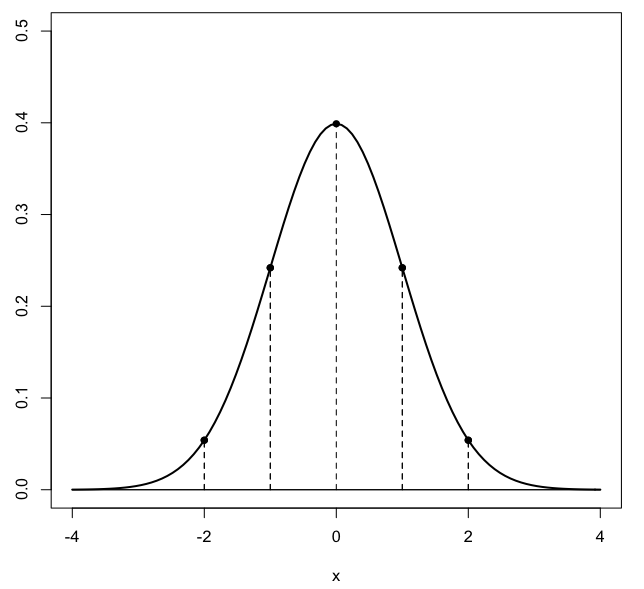
\includegraphics [scale=0.4] {gauss3.png} \end{center}

\title{Angle bisector}
\date{}

\begin{document}
\maketitle
\Large
In this write-up we will prove a theorem about the angle bisector.  We will prove it only for the case of an acute triangle, but it is true for any triangle.
\begin{center} 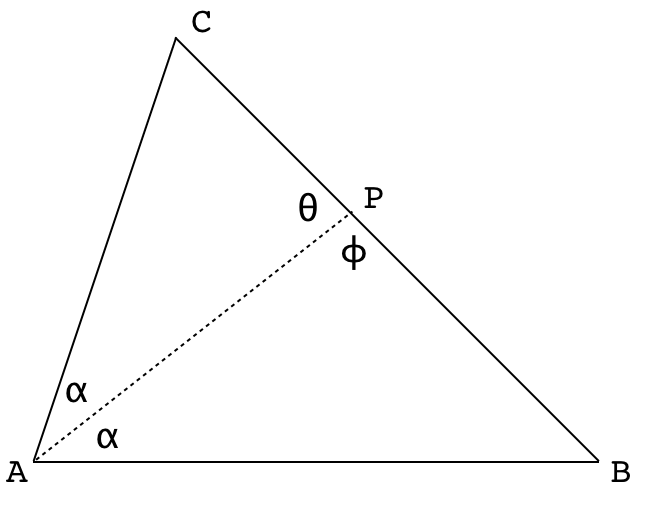
\includegraphics [scale=0.25] {angle_bisector1.png} \end{center}

Angle $A$ in $\triangle ABC$ is bisected by $AP$.  In general, the lengths $BP$ and $CP$ are not equal.  However, the ratios to their respective adjacent sides are equal:
\[ \frac{CP}{AC} = \frac{BP}{AB} \]

To prove this theorem, we use the law of sines, which says that for any triangle with vertices $A$, $B$ and $C$ and opposing sides $a$, $b$ and $c$:
\[ \frac{\sin A}{a} = \frac{\sin B}{b} = \frac{\sin C}{c} \]
Thus
\[ \frac{\sin \alpha}{CP} = \frac{\sin \theta}{AC} \]
\[ \frac{\sin \alpha}{BP} = \frac{\sin \phi}{AB} \]
Combining these two results and eliminating $\alpha$:
\[ \sin \phi \frac{BP}{AB} = \sin \theta \frac{CP}{AC} \]
But $\theta$ and $\phi$ are supplementary angles, so $\sin \theta = \sin \phi$ and we obtain
\[ \frac{BP}{AB} = \frac{CP}{AC} \]
which is what we wanted to prove.
\begin{center} 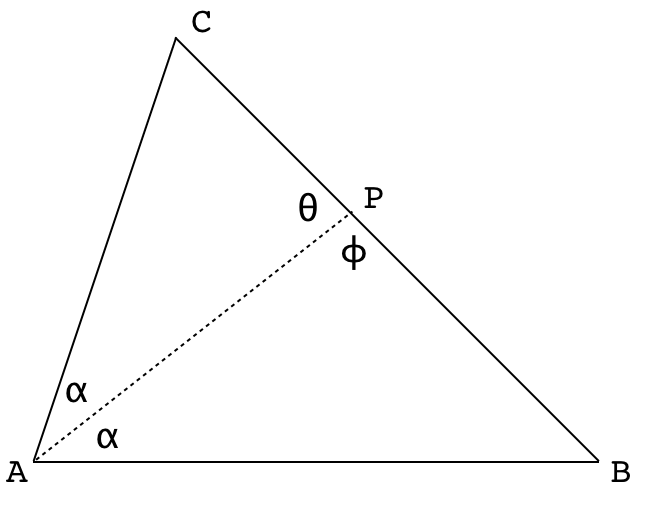
\includegraphics [scale=0.25] {angle_bisector1.png} \end{center}

The law of sines is easily demonstrated.  Drop an altitude in the triangle:
\begin{center} 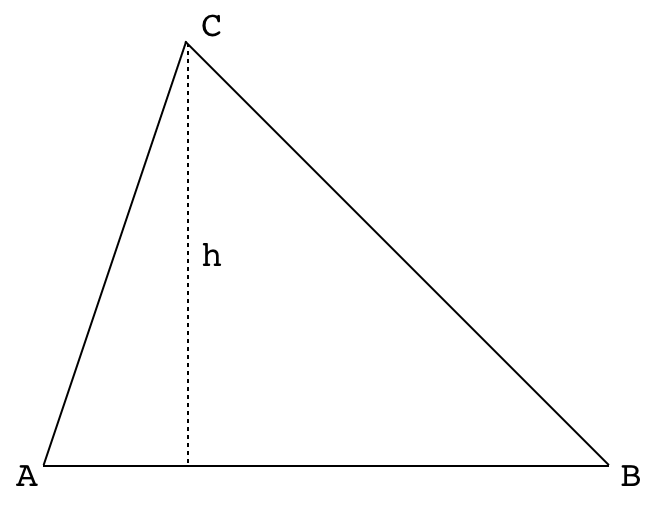
\includegraphics [scale=0.25] {angle_bisector2.png} \end{center}
\[ h = AC \sin A = BC \sin B \]
\[ \frac{\sin A}{BC} = \frac{\sin B}{AC} \]
By symmetry, the same can be done for angle-opposing side pair.

The other theorem we used is that the sines of supplementary angles are equal.  Suppose 
\[ \theta + \phi = 180 \]
\[ \theta = 180 - \phi \]
Then write the double-angle formula for sine:
\[ \sin 180 - \phi = \sin 180 \cos \phi - \sin \phi \cos 180 \]
\[ = 0 - \sin \phi \ (-1) = \sin \phi \]
Hence
\[ \sin \theta = \sin \phi \]
A simple construction of the angle $180 - \phi$ makes this obvious.
\begin{center} 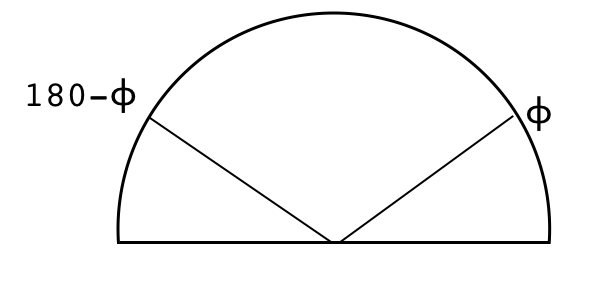
\includegraphics [scale=0.4] {angle_bisector3.png} \end{center}


\end{document}